% !TEX program = XeLaTeX
%%=======================================================================
%% HUAS-Beamer-EN.tex —— 湖南文理学院 Beamer 模板英文演示（暖色调，English demo）
%%=======================================================================
%% Compile: xelatex HUAS-Beamer-EN.tex
%%   (with references: xelatex -> bibtex -> xelatex x2)
%%
%% ★ How to adapt this template ★
%%   1. Cover info: edit \title / \subtitle / \author / \supervisor /
%%      \institute / \date below ([] = short title shown in the footer)
%%   2. Structure: \section (auto section page + TOC), \subsection,
%%      \begin{frame}{title}...\end{frame} = one slide
%%   3. Colors / sizes / figures / fonts: see ★调色★ / ★尺寸★ comments
%%      in huasbeamer.sty, or docs/模板使用与自定义说明.md
%%   4. All content below is layout showcase; replace it with yours
%%=======================================================================
\documentclass[aspectratio=169]{beamer} % 16:9; drop aspectratio for 4:3

% Figures (badge, logo, line-art buildings are in figures/)
\graphicspath{{figures/}}

% Load HUAS theme in English mode (options: en / notoc / subsectiontoc / nonav)
\usepackage[en]{huasbeamer}

% Common packages (add or remove as needed)
\usepackage{listings}
\usepackage{multicol}
\usepackage{multirow}

\lstset{
  basicstyle=\ttfamily\scriptsize,
  keywordstyle=\bfseries\color{huasdeep},
  commentstyle=\itshape\color{huascoral},
  stringstyle=\color{huasorange},
  numbers=left,
  numberstyle=\tiny\color{gray},
  frame=single,
  rulecolor=\color{huasred!40},
  breaklines=true,
  aboveskip=0.2ex,
  belowskip=0.2ex,
}

%% ---------------- Title Information (★ fill in your own ★) ----------------
\title[Self-directed Reading]{On the Teaching of Self-directed Reading Texts}
\subtitle{A Case Study of Units 2 \& 4, Grade 8 Chinese Textbook}
\author[Zhang San]{Presenter: Zhang San}
\supervisor{Supervisor: Prof. Li Si}
\institute[Hunan University of Arts and Science]{\small School of Literature, Hunan University of Arts and Science}
\date{\small June 2025}

\begin{document}

%% ---------------- Title Page ----------------
\begin{frame}[plain,noframenumbering]
  \titlepage
\end{frame}

%% ---------------- Outline ----------------
\begin{frame}{Contents}
  \tocbackground % TOC background: campus gate line-art (defined in huasbeamer.sty)
  \vskip-2em % ★位置★ move the overall TOC upward
  {\setbeamerfont{section in toc}{size=\large}% ★字号★ enlarge TOC entries
   \tableofcontents[hideallsubsections]}
\end{frame}

%% ==================== 1. Background ====================
\section{Background and Significance}

\subsection{Research Background}

\begin{frame}{Research Background}
  \begin{block}{Policy Context}
    \begin{itemize}
      \item The unified Chinese textbook builds a tripartite reading system:
            \emph{guided reading --- self-directed reading --- extensive reading};
      \item Self-directed texts bridge teacher guidance and autonomous reading;
      \item The curriculum standards emphasize independent reading competence.
    \end{itemize}
  \end{block}
  \begin{alertblock}{Practical Dilemmas}
    \begin{itemize}
      \item Self-directed texts are often taught exactly like guided ones;
      \item Students' agency is weak, and strategy transfer stays limited.
    \end{itemize}
  \end{alertblock}
\end{frame}

\subsection{Significance}

\begin{frame}{Significance}
  \begin{columns}[T]
    \begin{column}{0.48\textwidth}
      \begin{exampleblock}{Theoretical Value}
        \begin{itemize}
          \item Enriches research on self-directed text teaching;
          \item Grounds the tripartite reading system in practice.
        \end{itemize}
      \end{exampleblock}
    \end{column}
    \begin{column}{0.48\textwidth}
      \begin{exampleblock}{Practical Value}
        \begin{itemize}
          \item Offers actionable strategies for frontline teachers;
          \item Fosters autonomous construction of reading ability.
        \end{itemize}
      \end{exampleblock}
    \end{column}
  \end{columns}
  \vskip1ex
  {\footnotesize\color{huasdeep}%
    Cf. \emph{Chinese Curriculum Standards for Compulsory Education (2022)}
    \cite{xkb2022}.}
\end{frame}

%% ==================== 2. Contents and Methods ====================
\section{Contents and Methods}

\subsection{Research Contents}

\begin{frame}{Research Contents}
  \begin{itemize}[<+-| alert@+>]
    \item Analyze the arrangement of self-directed texts in Units 2 and 4;
    \item Investigate current teaching practices and problems;
    \item Propose principles and strategies for self-directed text teaching;
    \item Design lesson cases and reflect on classroom practice.
  \end{itemize}
  \vskip1.5ex
  \begin{block}{Key Concept}
    \emph{Self-directed text}: text types read mainly autonomously, with the
    teacher acting as a facilitator, emphasizing the transfer of reading
    strategies \cite{wang2019}.
  \end{block}
\end{frame}

\subsection{Methods}

\begin{frame}{Research Methods}
  \begin{table}
    \centering\small
    \caption{Overview of research methods}\label{tab:method-en}
    \begin{tabular}{lll}
      \huastableheader % colored header row (macro provided by huasbeamer)
      \huastableheaderfont Method & \huastableheaderfont Sample & \huastableheaderfont Purpose \\
      \midrule
      Literature review & 42 journal papers & Map the research field \\
      Questionnaire & 320 participants & Profile current practice \\
      Classroom observation & 12 lessons & Analyze teaching behavior \\
      Case analysis & 6 lesson designs & Distill practical strategies \\
      \bottomrule
    \end{tabular}
  \end{table}
\end{frame}

\subsection{Data Analysis Example}

\begin{frame}[fragile]{Data Analysis Example}
  \vspace{-1.2ex}
  \begin{block}{Survey statistics (excerpt)}
    Class-level means of reading self-efficacy ($n=320$):
    \begin{equation}
      \bar{X} = \frac{1}{n}\sum_{i=1}^{n} x_i,
      \qquad
      S = \sqrt{\frac{1}{n-1}\sum_{i=1}^{n}(x_i-\bar{X})^2}
      \label{eq:mean-en}
    \end{equation}
    Pre-post differences are examined with paired $t$-tests\cite{li2021}.
  \end{block}
  \vspace{-0.8ex}
  \begin{exampleblock}{Analysis script (excerpt)}
\begin{lstlisting}[language=Python]
import pandas as pd
data = pd.read_excel("reading_survey.xlsx")
mean, std = data["score"].mean(), data["score"].std()
print(f"mean = {mean:.2f}, std = {std:.2f}")
\end{lstlisting}
  \end{exampleblock}
\end{frame}

%% ==================== 3. Strategies and Practice ====================
\section{Strategies and Practice}

\subsection{Teaching Principles}

\begin{frame}{Principles of Self-directed Text Teaching}
  \begin{enumerate}
    \item \textbf{Student agency} --- give classroom time back to readers;
    \item \textbf{Strategy transfer} --- reuse strategies from guided reading;
    \item \textbf{Assessment-driven} --- task sheets and reading logs as engines;
    \item \textbf{Integration} --- link in-class self-directed reading with
          extensive reading.
  \end{enumerate}
  \vskip2ex
  \begin{block}{Side notes as scaffolding}
    The side notes in self-directed texts provide thinking scaffolds; teachers
    should help students \emph{learn to ask questions} with them until
    independent reading is achieved.
  \end{block}
\end{frame}

\subsection{Lesson Design}

\begin{frame}{Lesson Design: \emph{Return of the Wild Geese}}
  \begin{columns}[T]
    \begin{column}{0.52\textwidth}
      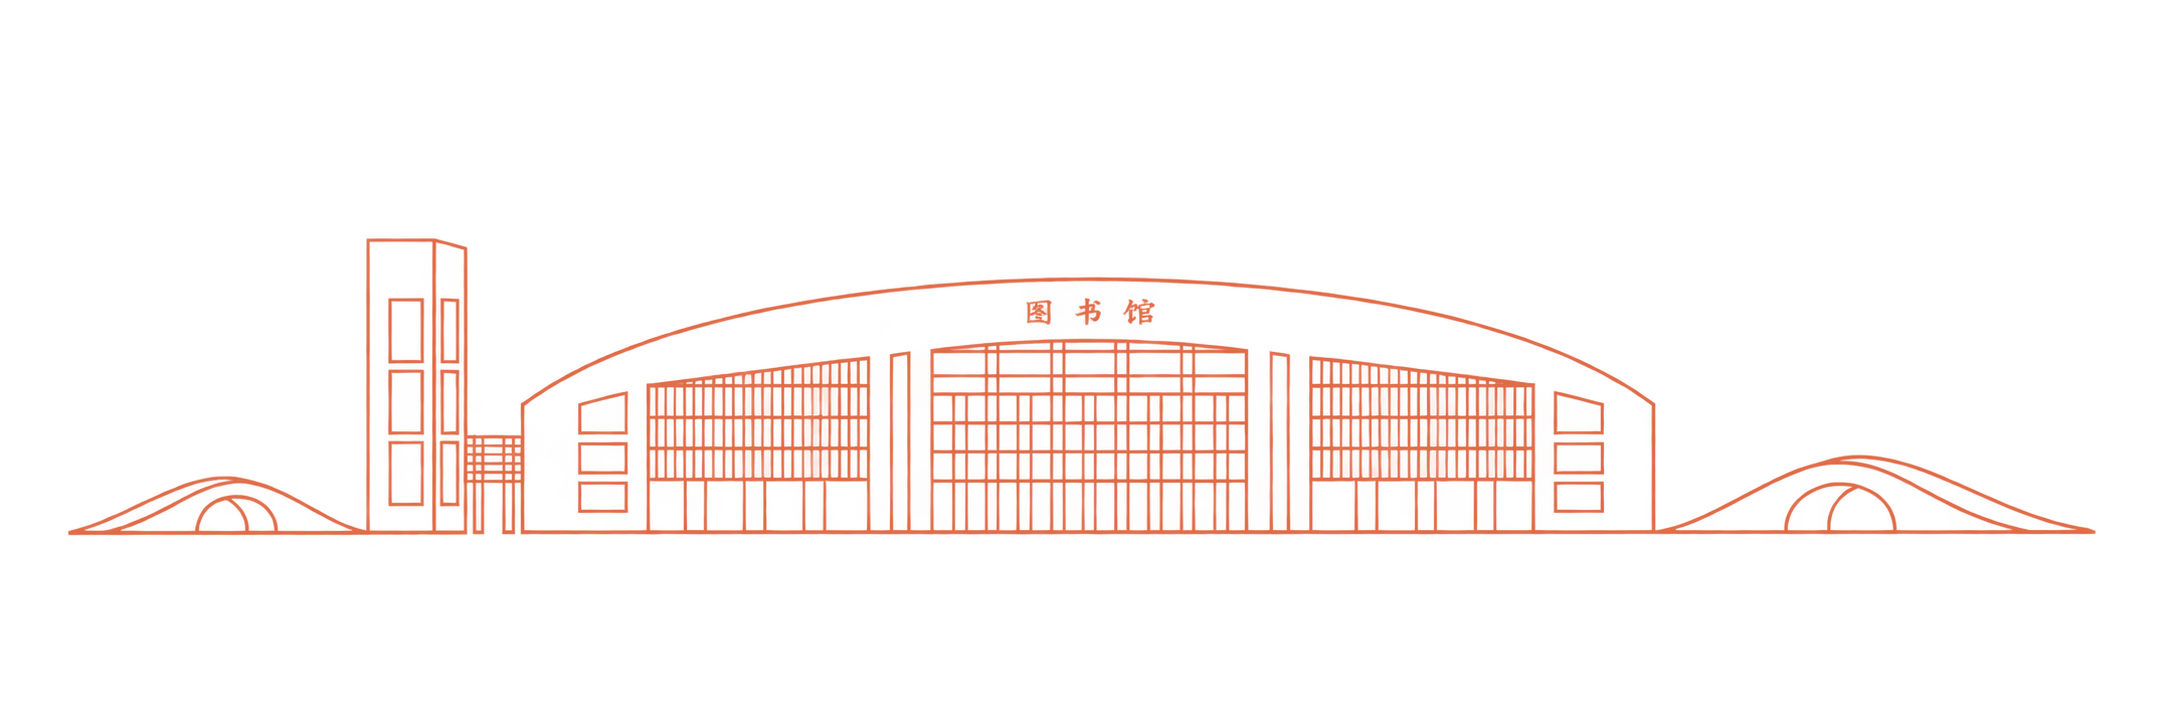
\includegraphics[width=\textwidth]{building-library.png}\\[0.5ex]
      {\scriptsize\color{huascoral}Fig.: Library of HUAS (illustrative material)}
    \end{column}
    \begin{column}{0.44\textwidth}
      \small
      \begin{description}
        \item[Lead-in] Short video on bird migration;
        \item[Reading] Task sheet with side notes;
        \item[Sharing] Group reports and peer questioning;
        \item[Transfer] Comparative reading of another text;
        \item[Homework] A 300-word observation note.
      \end{description}
    \end{column}
  \end{columns}
\end{frame}

\subsection{Practical Effects}

\begin{frame}{Practical Effects}
  \begin{block}{Classroom observation}
    \begin{itemize}
      \item Independent reading time rose from 8 to 18 minutes per lesson;
      \item Student-initiated questions grew from 21\% to 57\%;
      \item Completion rate of strategy-transfer tasks increased by 32\%.
    \end{itemize}
  \end{block}
  \begin{alertblock}{A caveat}
    Self-directed does not mean ``hands-off'': teacher feedback remains the
    guarantee of reading quality.
  \end{alertblock}
\end{frame}

%% ==================== 4. Conclusion ====================
\section{Conclusion and Outlook}

\begin{frame}{Conclusion and Outlook}
  \begin{block}{Conclusions}
    \begin{itemize}
      \item Self-directed text teaching should return to autonomous reading;
      \item Task sheets + side-note scaffolds + comparative reading work well;
      \item Integrated design of the tripartite reading system deserves study.
    \end{itemize}
  \end{block}
  \begin{exampleblock}{Future work}
    \begin{itemize}
      \item Quasi-experimental studies with larger samples;
      \item IT-supported assessment of self-directed classrooms.
    \end{itemize}
  \end{exampleblock}
\end{frame}

%% ---------------- References ----------------
\begin{frame}[allowframebreaks]{References}
  \footnotesize
  \bibliographystyle{plain}
  \bibliography{reference}
\end{frame}

%% ---------------- Acknowledgements / Q&A ----------------
\begin{frame}[plain,noframenumbering]
  \begin{tikzpicture}[remember picture,overlay]
    \shade[left color=huasdeep,right color=huasorange]
      (current page.south west) rectangle (current page.north east);
    \node[anchor=south,opacity=0.16] at ([yshift=0.35cm]current page.south) {%
      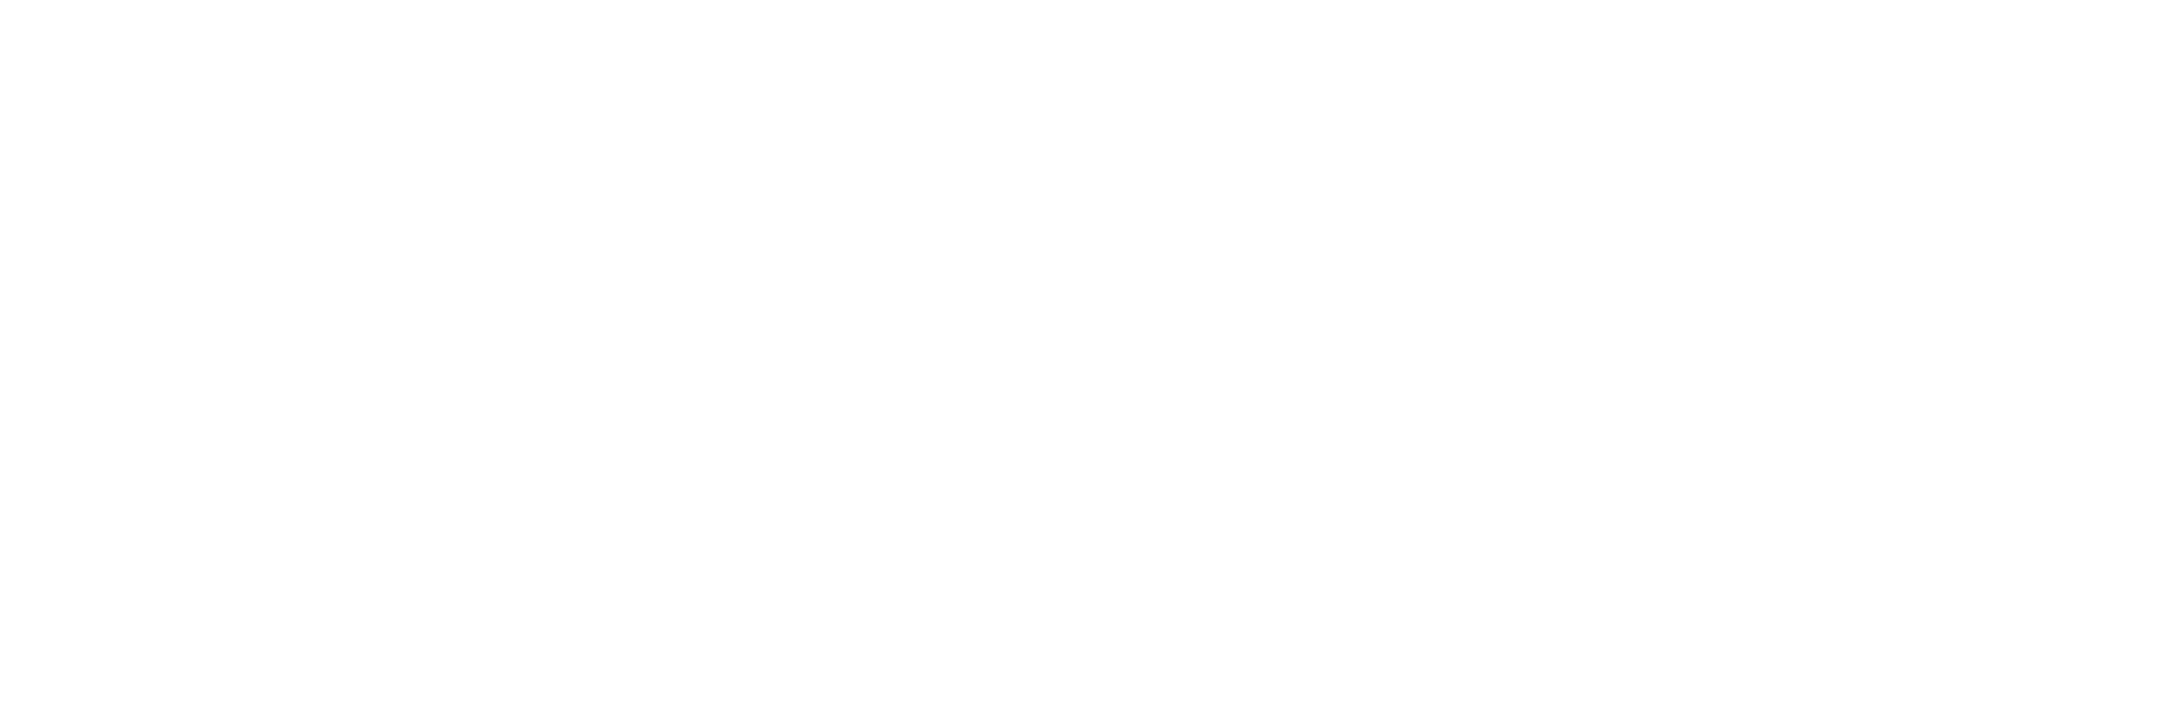
\includegraphics[width=1.04\paperwidth]{building-gate-white.png}};
  \end{tikzpicture}
  \vskip2.2cm
  \begin{center}
    {\Huge\bfseries\color{white}Thank You!}\\[1.8ex]
    {\large\color{white}Q \& A}\\[1.5ex]
    {\footnotesize\color{white!70}Hunan University of Arts and Science}
  \end{center}
\end{frame}

\end{document}
